\section{PROGRAMACIÓN COMPETITIVA}

Hay muchos tipos diferentes de concursos de programación en línea. El objetivo principal de tales concursos es permitir que concursantes o equipos de concursantes compitan. Los concursos pueden ser de muchos tipos diferentes: encontrar el algoritmo más eficiente, modelar un problema desafiante y escribir un programa para resolverlo, desarrollar un algoritmo de inteligencia artificial (IA) que se ejecute contra IA de otros concursantes. Además del concurso en sí y su objetivo principal, participar en dichos concursos también es una forma para que los concursantes aprendan y mejoren sus propias habilidades. Cuanto mejor y más relevante sea el apoyo al concursante y la retroalimentación recibida, más su aprendizaje será de buena calidad. Por ejemplo, proporcionar a los concursantes la solución correcta anotada con explicaciones al final del concurso, o permitirles participar en equipos puede mejorar su aprendizaje \citep{Combéfis-Wautelet}.

\subsection{INICIOS DE LOS CONCURSOS DE PROGRAMACIÓN COMPETITIVA}
La Competencia Internacional de Programación Universitaria (ICPC por sus siglas en inglés) se inician en 1970, cuando los pioneros de Alpha Chapter de la “Sociedad de honor de ciencias en computación” (UPE) presentaron la primera competencia de este estilo. La iniciativa se propagó rápidamente hacia los Estados Unidos y Canadá como un programa de innovación para incrementar ambición, aptitud de resolución de problemas, y la oportunidad para estudiantes fuertes en el campo de la computación \citep{icpc-glogal}.

Con el tiempo, el concurso se convirtió en una competencia de varios niveles con la primera ronda de campeonato realizada en 1977; desde entonces el concurso se ha expandido a una colaboración mundial de universidades que albergan competencias regionales que hacen avanzar a los equipos a la ronda anual de campeonato mundial, el ICPC World Finales \citep{icpc-glogal}.

El concurso internacional de programación universitaria, \textit{International Collegiate Programming Contest} (ICPC), es el concurso de programación más antiguo, más grande y más prestigioso del mundo. La ICPC tiene sus raíces en 1970, cuando los pioneros del Capítulo Alpha de la Sociedad de Honor de Ciencias de la Computación de la UPE organizaron la primera competencia. La iniciativa se extendió rápidamente dentro de los Estados Unidos y Canadá como un programa innovador para aumentar la ambición, la capacidad de resolución de problemas y las oportunidades de los estudiantes más fuertes en el campo de la informática. Con el tiempo, el concurso se convirtió en una competencia de varios niveles con la primera ronda de campeonato realizada en 1977. Desde entonces, el concurso se ha expandido a una colaboración mundial de universidades que organizan competiciones regionales que llevan a los equipos a la ronda anual de campeonato mundial, la ICPC World Final \citep{icpc-glogal}.

\begin{figure}[H]
    \centering
    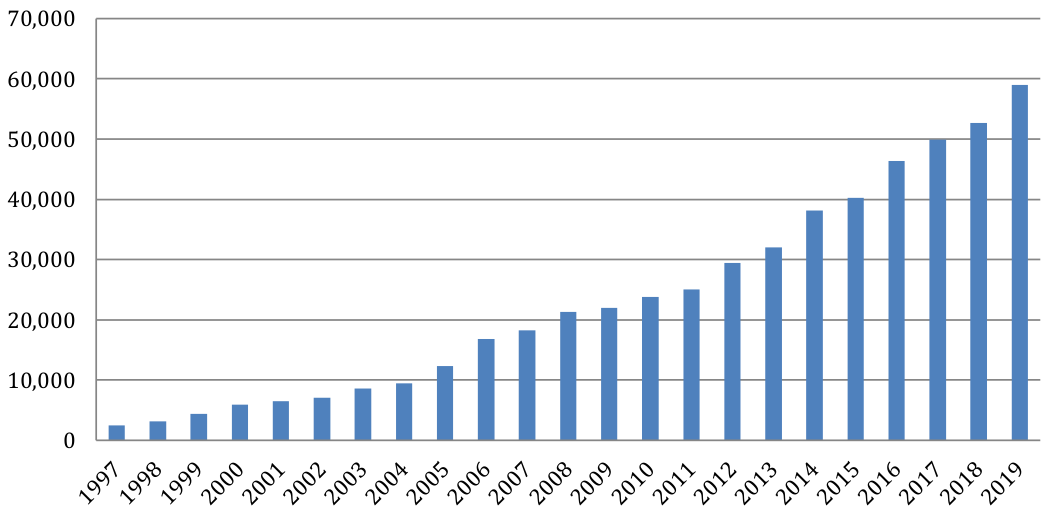
\includegraphics[scale=0.7]{imagenes/ICPC_student_participation.png}
    \caption{Participación de estudiantes en la ICPC\\ Fuente: \citep{icpc-glogal}}
\end{figure}

El concurso fomenta la creatividad, el trabajo en equipo y la innovación en la creación de nuevos programas de software, y permite a los estudiantes probar su capacidad para desempeñarse bajo presión. El concurso ha elevado las aspiraciones y el rendimiento de generaciones de solucionadores de problemas del mundo en ciencias de la computación e ingeniería. La ICPC presenta varios niveles de competencia:  

\begin{itemize}
    \item Campeonato Interno por Universidad
    \item Campeonato Departamental/Estatal. 
    \item Campeonato Nacional. 
    \item Campeonato Regional.
    \item Final Mundial. 
\end{itemize}

Los participantes conforman equipos de tres personas, cada equipo representa a su universidad y país respectivamente. El concurso dura cinco horas, tiempo en que los estudiantes deben resolver de ocho a trece problemas algorítmicos. Un equipo es ganador cuando éste resuelve la mayor cantidad de problemas en el menor tiempo de penalización (Wasik et al. 2018).

\subsection{PROGRAMACIÓN COMPETITIVA EN LATINOAMERICA}

En Bolivia también se llevan a cabo las competencias de programación competitiva, entre estos tenemos:
\begin{itemize}
    \item Olimpiadas Bolivianas en Informática (OBI): Se fundaron el año 2011, estas Olimpiadas están orientadas a niños de tercero hasta sexto de secundaria donde los primeros veinte clasificados pasan a formar un equipo que después de un año de capacitación compiten para los cuatro puestos para representar a Bolivia en la competencia \textit{International Olympiad in Informatics} (IOI)
    \item Red de programación competitiva (RPC): Se fundó hace siete años en Colombia, en el cual, cualquier persona o grupos de tres personas pueden inscribirse libremente y participar, la evaluación es de la misma modalidad de la ICPC. Cada una de las universidades bolivianas tienen una sede dentro del concurso, suele llevarse a cabo en tiempo real junto con otras universidades latinoamericanas. Este concurso se realiza cada 3 semanas aproximadamente.
    \item Torne Argentino de Programación (TAP): Es una competencia por equipos de 3 estudiantes de la misma institución de educación superior de Argentina. La competencia tiene 5 horas de duración, en las que cada equipo deberá resolver un conjunto de problemas algorítmicos, creando un programa que solucione cada problema, la evaluación es de la misma modalidad de la ICPC, este concurso se celebra cada año y sirve como un clasificatorio para los concursantes Argentinos a la fase Latinoamericana de Programación.
\end{itemize}

\subsection{JUEZ}

La clave principal para este tipo de concursos anteriormente mencionados es el sistema que verifica automáticamente la corrección de las soluciones presentadas por los participantes, también verifica que la solución no exceda los límites de utilización de recursos (como el tiempo y la memoria). Según la evaluación realizada, se calcula la clasificación en línea de todos los participantes presentado en tiempo real durante el desarrollo de un concurso.

El término juez fue introducido por primera vez el año 2001 por Kurnia, Lim y Cheang como una plataforma en línea que está inspirada tanto para las competencias de programación como para la educación. Kurnia, Lim y Cheang le dan forma a esta definición como una plataforma que puede evaluar automáticamente cualquier programa escrito en cierto lenguaje de programación en tiempo real. \citep{KURNIA2001299}

En general, el objetivo de los sistemas de jueces en línea es evaluar los programas algorítmicos de manera segura, confiable y continua.
A continuación se describe el proceso de evaluación:

1) Envío,

2) Evaluación

3) Puntuación.

Para cada ejecución de caso de prueba de la presentación particular, se verifica si:

1) El proceso de ejecución se realizó sin errores.

2) No se han excedido las limitaciones de recursos específicos del problema.

3) El resultado obtenido cumple con las reglas descritas en la definición del problema (Wasik et al. 2018).

En la actualidad, existen plataformas en línea que comparten desafíos similares a los que se utilizan para las competencias de programación, muchas universidades proveen este tipo de
sistemas para apoyar a sus estudiantes para la preparación de los concursos de programación.
\begin{itemize}
    \item \textit{UVa Online Judge}: Este juez en línea tiene sus inicios en noviembre de 1995, fue desarrollado inicialmente por un estudiante de informática para una competencia de programación que se iba a realizar en la Universidad de Valladolid en España; con el tiempo ese juez llegó a ser perfeccionado y ya no sólo se le utilizaba para las competencias de programación, sino también para el entrenamiento constante de los competidores del mundo ya que éste tenía una gran cantidad de desafíos de programación competitiva. Es el repositorio oficial para los problemas del ICPC , competencias regionales y la de los mundiales de programación (Revilla et al, 2018).
    \item Codeforces: Tiene sus inicios en el año 2010, su fundador es Mike Mirzayanov. Este juez en línea es uno de los más populares a nivel mundial, en un inicio fue preparado para los concursantes de nacionalidad rusa. Su forma de evaluación consiste en dos divisiones según su calificación de Elo, que se actualiza para cada competencia realizada \citep{codeforces}.
    \item SPOJ: Sphere Online Judge, es un juez en línea que tiene diversos desafíos de programación de todo tipo de nivel y se los puede clasificar mediante etiquetas \citep{spoj}.
    \item TopCoder: Es una empresa con comunidad global abierta de diseñadores, desarrolladores, científicos de datos, y programadores competitivos. En programación competitiva, topcoder gira alrededor de una ronda de competencias en su plataforma de juzgamiento SRM cronometrados de 1,5 horas en el que todos los participantes compiten en línea que tratan de resolver el mismo conjunto de problemas tan rápidamente como sea posible. Estos fueron el primer tipo de desafíos en Topcoder \citep{topcoder}.
    \item Codechef: Tiene sus inicios en septiembre de 2009 en Mumbai India. Se creó como una plataforma para ayudar a los programadores a triunfar en el mundo de los algoritmos, la programación de computadoras y los concursos de programación.
    En CodeChef se organiza un concurso de programación a principios de mes y dos desafíos de programación más pequeños a mediados y finales de mes. Esta plataforma también tiene sesiones de capacitación y discusiones relacionadas con algoritmos, búsqueda binaria, tecnicismos como el tamaño de la matriz y los gustos. Y como complemento final, la plataforma tiene varios documentos de algoritmos y debates en foros para ayudar a aquellos que son nuevos en el mundo de la programación de computadoras \citep{codechef}.
\end{itemize}

\section{CONTENIDO EN COMPETENCIAS DE PROGRAMACIÓN COMPETITIVA}
\changelocaltocdepth{2}
\subsection{Introducción}
\subsubsection{Conceptos}
La programación competitiva es una actividad que consiste en resolver problemas algorítmicos bajo ciertas restricciones de tiempo y espacio. Los competidores deben diseñar algoritmos eficientes para solucionar problemas específicos dentro de un tiempo limitado \cite{skiena2008algorithm}.
\paragraph{Lenguaje de Programación}
El lenguaje de programación es una herramienta fundamental para resolver problemas. Los lenguajes más utilizados en la programación competitiva incluyen C++, Java y Python, debido a su eficiencia y versatilidad \cite{stroustrup2013c++}.
\paragraph{Programación Competitiva}
La programación competitiva se basa en la capacidad de diseñar algoritmos eficientes y optimizar el uso de recursos. Es una disciplina que ayuda a mejorar las habilidades de resolución de problemas y el pensamiento lógico \cite{ahmed2020competitive}.
\paragraph{Herramientas}
Existen varias herramientas que facilitan la práctica de la programación competitiva, como compiladores, entornos de desarrollo integrado (IDE) y sistemas de control de versiones \cite{menezes2018tools}.

\subsubsection{Jueces}
Los jueces son plataformas en línea que permiten a los programadores competir y verificar la corrección de sus soluciones. Ejemplos populares incluyen Codeforces, LeetCode y HackerRank \cite{leon2017online}.

\subsubsection{Configuración del entorno de programación}
Un entorno de programación adecuado es crucial para la eficiencia en la resolución de problemas. Esto incluye la instalación de un buen IDE, la configuración de compiladores y la familiarización con las herramientas de depuración \cite{gaddis2018starting}.

\subsection{Fundamento de C++}
\subsubsection{Proceso de desarrollo de un programa}
El desarrollo de un programa en C++ sigue un proceso estructurado que incluye la planificación, codificación, prueba y depuración. Este proceso asegura que el código sea eficiente y libre de errores \cite{stroustrup2013c++}.

\subsubsection{Sintaxis}
La sintaxis de C++ define las reglas y estructuras que rigen la escritura del código. Es fundamental conocer la sintaxis para evitar errores de compilación y ejecución \cite{stroustrup2013c++}.

\subsubsection{Datos primitivos}
Los datos primitivos son los tipos de datos básicos que se utilizan en la programación. Estos incluyen booleanos, caracteres, enteros y punto flotante \cite{gaddis2018starting}.
\paragraph{Booleanos}
Los booleanos son tipos de datos que pueden tener dos valores: verdadero o falso.
\paragraph{Caracteres}
Los caracteres representan símbolos individuales, como letras y dígitos.
\paragraph{Enteros}
Los enteros son números sin parte decimal.
\paragraph{Punto flotante}
Los números de punto flotante representan números con parte decimal.

\subsubsection{Variables y constantes}
Las variables y constantes son elementos fundamentales para almacenar y manipular datos. Las variables pueden cambiar su valor durante la ejecución del programa, mientras que las constantes mantienen un valor fijo \cite{stroustrup2013c++}.

\subsubsection{Lectura e impresión}
La entrada y salida de datos son esenciales para la interacción con el usuario. En C++, se utilizan las funciones `cin` y `cout` para la lectura e impresión de datos, respectivamente \cite{gaddis2018starting}.

\subsubsection{Operadores}
Los operadores permiten realizar operaciones sobre los datos. Estos incluyen operadores aritméticos, de asignación, de relación y lógicos \cite{stroustrup2013c++}.
\paragraph{Operadores aritméticos}
Los operadores aritméticos se utilizan para realizar operaciones matemáticas básicas como suma, resta, multiplicación y división.
\paragraph{Operadores de asignación}
Los operadores de asignación se utilizan para asignar valores a las variables.
\paragraph{Operadores de relación}
Los operadores de relación se utilizan para comparar dos valores y devuelven un valor booleano.
\paragraph{Operadores lógicos}
Los operadores lógicos se utilizan para combinar expresiones booleanas.

\subsubsection{Estructuras de Control}
Las estructuras de control permiten dirigir el flujo de ejecución del programa. Estas incluyen sentencias de decisión, iteración y las sentencias `break` y `continue` \cite{gaddis2018starting}.
\paragraph{Sentencias de decisión}
Las sentencias de decisión, como `if` y `switch`, permiten ejecutar diferentes bloques de código según ciertas condiciones.
\paragraph{Sentencias de iteración}
Las sentencias de iteración, como `for` y `while`, permiten repetir bloques de código varias veces.
\paragraph{Sentencias Break y Continue}
Las sentencias `break` y `continue` se utilizan para controlar la ejecución de bucles.

\subsubsection{Misceláneas}
En esta sección se abarcan otros temas varios relacionados con la programación en C++.

\subsection{Estructura de datos}
\subsubsection{Estructura de datos estáticas simples}
Las estructuras de datos estáticas simples incluyen booleanos, caracteres, enteros y punto flotante. Estas estructuras son fundamentales para el almacenamiento y manipulación de datos \cite{gaddis2018starting}.
\paragraph{Booleanos}
\paragraph{Caracteres}
\paragraph{Enteros}
\paragraph{Punto flotante}

\subsubsection{Estructura de datos estáticas compuestas}
Las estructuras de datos estáticas compuestas incluyen arreglos, matrices, arreglos multidimensionales, pares, tuplas y `struct`. Estas estructuras permiten almacenar colecciones de datos relacionados \cite{stroustrup2013c++}.
\paragraph{Arreglos}
\paragraph{Matrices}
\paragraph{Arreglos multidimensionales}
\paragraph{Pares}
\paragraph{Tuplas}
\paragraph{Struct}

\subsubsection{Estructura de datos dinámicas lineales}
Las estructuras de datos dinámicas lineales incluyen cadenas, vectores, pilas, colas y colas dobles. Estas estructuras permiten la manipulación dinámica de datos \cite{stroustrup2013c++}.
\paragraph{Cadenas}
\paragraph{Vectores}
\paragraph{Pilas}
\paragraph{Colas}
\paragraph{Colas dobles}

\subsubsection{Estructura de datos dinámicas no lineales}
Las estructuras de datos dinámicas no lineales incluyen colas de prioridad, conjuntos y mapas. Estas estructuras permiten la organización y acceso eficiente a los datos \cite{stroustrup2013c++}.
\paragraph{Colas de prioridad}
\paragraph{Conjuntos}
\paragraph{Mapas}

\subsection{Programación modular}
\subsubsection{Funciones y Métodos}
Las funciones y métodos son bloques de código reutilizables que realizan tareas específicas. Pueden recibir parámetros como valor o referencia \cite{stroustrup2013c++}.
\paragraph{Parámetros como valor y referencia}
\subsubsection{Recursividad}
La recursividad es una técnica en la que una función se llama a sí misma para resolver problemas más pequeños del mismo tipo.

\subsection{Matemáticas I}
\subsubsection{Progresiones}
Las progresiones son secuencias de números con una relación definida entre ellos. Incluyen progresiones aritméticas y geométricas \cite{skiena2008algorithm}.
\paragraph{Progresiones aritméticas}
\paragraph{Progresiones geométricas}
\paragraph{Otras progresiones}
\subsubsection{Sucesiones}
Las sucesiones son secuencias de números generados según una regla específica. Ejemplos incluyen la sucesión de Fibonacci y la sucesión de números primos \cite{ahmed2020competitive}.
\paragraph{Sucesión Fibonacci}
\paragraph{Sucesión de números primos}
\paragraph{Otras sucesiones}
\subsubsection{Números figurados}
Los números figurados representan figuras geométricas y se clasifican en números poligonales, poligonales centrados y poliédricos.
\paragraph{Números poligonales}
\paragraph{Números poligonales centrados}
\paragraph{Números poliédricos}
\subsubsection{Permutaciones}
Las permutaciones son arreglos de elementos en un orden específico.
\subsubsection{Combinaciones}
Las combinaciones son selecciones de elementos sin importar el orden.

\subsection{Complejidad Algorítmica}
La complejidad algorítmica mide la eficiencia de un algoritmo en términos de tiempo y espacio. Es fundamental para evaluar el rendimiento de los algoritmos \cite{skiena2008algorithm}.

\subsection{Bits}
\subsubsection{Base binaria}
La base binaria es un sistema numérico que utiliza solo dos dígitos: 0 y 1. Es la base de la informática digital \cite{gaddis2018starting}.
\subsubsection{Representación de enteros y punto flotante}
La representación de enteros y punto flotante en binario permite el almacenamiento y manipulación de números en computadoras.
\subsubsection{Operadores binarios bit a bit}
Los operadores binarios bit a bit realizan operaciones sobre los bits individuales de los operandos.
\subsubsection{Operadores de desplazamiento de bits}
Los operadores de desplazamiento de bits mueven los bits a la izquierda o a la derecha, cambiando el valor numérico.
\subsubsection{Aplicaciones de los operadores}
Los operadores binarios se utilizan en aplicaciones como criptografía y compresión de datos.
\subsubsection{Máscara de bits}
Las máscaras de bits se utilizan para manipular bits específicos dentro de un valor binario.

\subsection{Matemáticas II}
\subsubsection{Números primos}
Los números primos son aquellos que solo tienen dos divisores: 1 y ellos mismos. Son fundamentales en teoría de números y criptografía \cite{ahmed2020competitive}.
\paragraph{Prueba de primalidad}
La prueba de primalidad es un algoritmo para determinar si un número es primo.
\subsubsection{Criba de Eratóstenes}
La criba de Eratóstenes es un algoritmo eficiente para encontrar todos los números primos menores que un número dado.
\subsubsection{Factorización de enteros}
La factorización de enteros descompone un número en sus factores primos.
\paragraph{Criba extendida}
La criba extendida es una versión mejorada de la criba de Eratóstenes para encontrar factores primos.
\subsubsection{MCD y MCM}
El máximo común divisor (MCD) y el mínimo común múltiplo (MCM) son operaciones fundamentales en teoría de números.
\subsubsection{Aritmética modular}
La aritmética modular es un sistema de aritmética para números enteros donde los números “vuelven a empezar” después de alcanzar un valor fijo, llamado módulo.
\subsubsection{Exponenciación binaria}
La exponenciación binaria es un método rápido para calcular potencias grandes de un número.
\subsubsection{Teorema extendido de Euclides}
El teorema extendido de Euclides es una extensión del algoritmo de Euclides para encontrar el MCD, y también encuentra los coeficientes que satisfacen la identidad de Bézout.

\subsection{Algoritmos I}
\subsubsection{Problemas Ad Hoc}
Los problemas Ad Hoc son problemas únicos que no se ajustan a ninguna categoría específica y requieren soluciones específicas \cite{ahmed2020competitive}.
\subsubsection{Ordenamientos}
Los algoritmos de ordenamiento organizan los elementos de una lista en un orden específico. Incluyen el ordenamiento rápido, por mezcla, por montículos y por cuentas \cite{skiena2008algorithm}.
\paragraph{Ordenamiento rápido}
\paragraph{Ordenamiento por mezcla}
\paragraph{Ordenamiento por montículos}
\paragraph{Ordenamiento por cuentas}
\subsubsection{Búsqueda binaria}
La búsqueda binaria es un algoritmo eficiente para encontrar un elemento en una lista ordenada.
\subsubsection{Max Sum 1D y 2D}
Los algoritmos Max Sum encuentran la submatriz de suma máxima en matrices unidimensionales y bidimensionales.

\subsection{Grafos I}
\subsubsection{Clasificación}
Los grafos se clasifican en dirigidos y no dirigidos, y se utilizan para representar relaciones entre objetos \cite{skiena2008algorithm}.
\subsubsection{Representación de grafos}
Los grafos se pueden representar mediante matrices de adyacencia o listas de adyacencia.
\subsubsection{Recorridos}
Los recorridos en grafos incluyen el recorrido en profundidad (DFS) y el recorrido en anchura (BFS).
\paragraph{DFS}
\paragraph{BFS}
\subsubsection{Flood Fill}
El algoritmo Flood Fill se utiliza para determinar las áreas conectadas en una matriz.
\subsubsection{Orden Topológico}
El orden topológico de un grafo dirigido acíclico (DAG) es una ordenación de sus vértices que respeta las relaciones de precedencia.

\subsection{Estructura de datos II}
\subsubsection{Union Find}
El algoritmo Union Find es una estructura de datos para manejar particiones dinámicas de un conjunto.
\subsubsection{Montículos}
Los montículos son estructuras de datos que permiten la extracción eficiente del valor mínimo o máximo.
\subsubsection{Árbol de segmentos}
El árbol de segmentos es una estructura de datos que permite consultas rápidas sobre intervalos de un arreglo.
\subsubsection{Tabla dispersa}
La tabla dispersa es una estructura de datos que permite resolver consultas de rango estáticas.
\subsubsection{Árbol de Fenwick}
El árbol de Fenwick es una estructura de datos que permite la actualización y consulta eficiente de sumas de prefijos.

\subsection{Grafos II}
\subsubsection{Árbol de expansión mínima}
El árbol de expansión mínima es un subgrafo que conecta todos los vértices con el peso mínimo total \cite{skiena2008algorithm}.
\paragraph{Kruskal}
\paragraph{Prim}
\subsubsection{Caminos más cortos}
Los algoritmos de caminos más cortos encuentran la ruta mínima entre dos vértices en un grafo.
\paragraph{Dijkstra}
\paragraph{Dijkstra chino}
\paragraph{Bellman-Ford}
\paragraph{Floyd-Warshall}
\subsubsection{Puentes y puntos de articulación}
Los puentes y puntos de articulación son aristas y vértices cuya eliminación aumenta el número de componentes conectados del grafo.
\subsubsection{Componentes Conexas}
Las componentes conexas son subgrafos en los que cualquier par de vértices está conectado.
\paragraph{Tarjan}
\paragraph{Kosaraju}

\subsection{Programación Dinámica}
\subsubsection{Introducción}
La programación dinámica es una técnica de optimización que resuelve problemas dividiéndolos en subproblemas más pequeños \cite{ahmed2020competitive}.
\subsubsection{La subsecuencia creciente más larga (LIS)}
La subsecuencia creciente más larga es el problema de encontrar una subsecuencia de un arreglo donde los elementos estén en orden creciente.
\subsubsection{La subsecuencia común más larga (LCS)}
La subsecuencia común más larga encuentra la subsecuencia más larga que es común a dos secuencias.
\subsubsection{Mínima edición de distancia}
La mínima edición de distancia mide el número mínimo de operaciones necesarias para convertir una cadena en otra.
\subsubsection{Problema de la mochila}
El problema de la mochila busca maximizar el valor total de los objetos en una mochila con capacidad limitada.
\subsubsection{Problema de cambio de moneda}
El problema de cambio de moneda encuentra la forma de hacer cambio para un monto específico con la menor cantidad de monedas posible.
\subsubsection{Backtracking}
El backtracking es una técnica para resolver problemas recursivamente probando todas las posibles soluciones y retrocediendo cuando una solución no es válida.
\subsubsection{El problema del viajero (TSP)}
El problema del viajero encuentra el camino más corto que visita un conjunto de ciudades y vuelve a la ciudad de origen.
\subsubsection{Otros problemas de programación dinámica}

\subsection{Algoritmos de cadenas}
\subsubsection{Algoritmo Z}
El algoritmo Z encuentra todas las ocurrencias de un patrón en un texto.
\subsubsection{Algoritmo Knuth-Morris-Pratt}
El algoritmo Knuth-Morris-Pratt (KMP) encuentra todas las ocurrencias de un patrón en un texto de manera eficiente.
\subsubsection{Trie}
El trie es una estructura de datos que almacena un conjunto de cadenas, permitiendo búsquedas rápidas.
\subsubsection{Hashing}
El hashing convierte entradas en valores únicos, usados para búsquedas y almacenamiento eficientes.

\subsection{Algoritmos II}
\subsubsection{Técnica Divide y Vencerás}
La técnica divide y vencerás divide un problema en subproblemas más pequeños y los resuelve recursivamente.
\subsubsection{Algoritmos voraces}
Los algoritmos voraces toman decisiones óptimas locales para encontrar una solución global.
\subsubsection{Teoría de juegos}
La teoría de juegos estudia estrategias óptimas en juegos de decisión.
\subsubsection{Sliding Window}
La técnica de sliding window mantiene un rango de elementos en una secuencia, utilizado para resolver problemas de intervalos.
\subsubsection{Meet in the Middle}
La técnica meet in the middle divide el problema en dos partes para reducir la complejidad de la búsqueda.

\subsection{Grafos III}
\subsubsection{Ancestro Común más bajo}
El ancestro común más bajo es el nodo más bajo en un árbol que tiene dos nodos dados como descendientes.
\subsubsection{Maximum bipartite matching}
El emparejamiento bipartito máximo encuentra el mayor conjunto de emparejamientos en un grafo bipartito.
\subsubsection{Flujos}
Los algoritmos de flujos encuentran el flujo máximo en una red de flujo.
\subsubsection{Heavy Light Decomposition}
La descomposición heavy light divide un árbol en caminos para responder a consultas de rango de manera eficiente.

\subsection{Geometría Computacional}
\subsubsection{Representación de elementos}
La representación de elementos geométricos incluye puntos, líneas y polígonos.
\subsubsection{Producto cruz y producto punto}
El producto cruz y el producto punto son operaciones fundamentales en geometría computacional.
\subsubsection{Intersección de elementos}
La intersección de elementos determina si dos elementos geométricos se cruzan.
\subsubsection{Sweep Line}
El algoritmo sweep line resuelve problemas geométricos mediante el barrido de una línea a través del plano.
\subsubsection{Otros problemas}
Esta sección incluye otros problemas diversos en geometría computacional.
\changelocaltocdepth{4}